%%%%%%%%%% DOCUMENT STUFF %%%%%%%%%%

\documentclass[10.5pt,letterpaper]{article}
\usepackage{mathtools}
\usepackage{amsmath}
\usepackage{amssymb}
\usepackage{datetime}
\usepackage{setspace}
\usepackage{tikz}
\usepackage[margin=1in]{geometry}
\usepackage{courier}
\usepackage{listings}
\usepackage{mips}
\usepackage{graphicx}
\usepackage{enumitem}
\usepackage{pgfplots}
\usepackage{colortbl}
\usepackage{mdframed}
\usepackage{xcolor}
\usepackage{fancybox}

%%%%%%%%%% FORMATTING %%%%%%%%%%

\newdate{date}{03}{12}{2017}
\spacing{1.5}
\date{\displaydate{date}}
\setcounter{secnumdepth}{0}
\newcommand\tab[1][0.5cm]{\hspace*{#1}}
\newcommand*\circled[1]{\tikz[baseline=(char.base)]{
            \node[shape=circle,draw,inner sep=2pt] (char) {#1};}}
\usetikzlibrary{arrows.meta,shapes,automata,petri,positioning,calc}

\tikzset{
    place/.style={
        circle,
        thick,
        draw=black,
        minimum size=6mm,
    },
        state/.style={
        circle,
        thick,
        draw=black!75,
        %fill=green!20,
        minimum size=6mm,
    },
}

\graphicspath{{images/}}

%%%%%%%%%% CONTENT %%%%%%%%%%

%%%%% COVER PAGE %%%%%

\begin{document}
\title{CS 161: Homework 8}
\author{
	Jonathan Woong\\
	804205763\\
	Fall 2017\\
	Discussion 1A}
\maketitle
\pagebreak

%%%%% PROBLEMS %%%%%

\begin{enumerate}[label=\textbf{Problem \arabic*.}]
\item Conisder the following problem which was discussed in class: \\
Suppose that we have a patient who was just tested for a particular disease and the test came out positive. We know that one in every thousand people has this disease. We also know that the test is not reliable: it has a false positive rate of 2\% and a false negative rate of 5\%. Our goal is then to assess our belief in the patient having the disease given that the test came out positive. If we let the propositional variable D stand for the patient has the disease, and the propositional variable T stand for the test came out positive, our goal is then to compute $Pr(D|T)$.\\
You may also recall being surprised that $Pr(D|T)\approx 0.045$. The goal of this question is then to identify conditions under which this probability will be no less than 0.30. You will need to find the answer to this by constructing a Bayesian Network and using the sensitivity engine of SamIam.\\\\
By constraining $Pr(T)$ to always be true, running the sensitivity analysis on the $Pr(D|T)$ with the constraint $Pr(D|T)\geq 0.3$ gives the following suggested parameters:
\[\begin{tabular} {|c|c|c|}
\hline
\textbf{Parameter} & \textbf{Current Value} & \textbf{Suggested Value} \\
\hline
$Pr(D)$ & 0.001 & $\geq 0.008942$ \\
\hline
$Pr(T|\lnot D)$ & 0.02 & $\leq 0.00219$ \\
\hline
\end{tabular}\]
\item Consider the folowing scenario:\\
When Sambot goes home at night, he wants to know if his family is home before he tries the doors. (Perhaps the most convenient door ot enter is double locked when nobody is home). Often when Sambots wife leaves the house she turns on an outdoor light. However, she sometimes turns on this light if she is expecting a guest. Also, Sambots family has a dog. When nobody is home, the dog is put in the backyard. The same is true if the dog has bowel trouble. Finally, if the dog is in the backyard, Sambot will probably hear her barking, but sometimes he can be confused by other dogs barking. Sambot is equipped with two sensors: a light-sensor for detecting outdoor lights and a sound-sensor for detecting the barking of the dog(s). BOth of these sensors are not completely reliable and can break. Moreover, they both require Sambots battery to be in good condition.\\
Your task is to build a belief network that Sambot will use to reason about the above situation using the modeling and inference tool SamIam. Specifically, given sensory input, Sambot needs to compute his beliefs in various events: whether his family is home, whether any of his sensors are broken, whether the dog is in the backyard, and whether it has bowel trouble.\\
You need to proceed as follows:
	\begin{enumerate}[label=(\alph*)]
	\item Decide on the set of variables and their values. These variables and values must match those in the given data file sambot.dat.
	\[\begin{tabular}{|c|c|}
	\hline
	\textbf{Variable} & \textbf{Possible Values} \\
	\hline
	ExpectingGuests & Yes, No, N/A \\
	\hline
	FamilyHome & Yes, No, N/A \\
	\hline
	SoundSensor & On, Off, N/A \\
	\hline
	LightSensor & On, Off, N/A \\
	\hline
	HearableBarking & Yes, No, N/A \\
	\hline
	Battery & OK, Dead, N/A \\
	\hline
	SoundSensorHealth & OK, Broken, N/A \\
	\hline
	LightSensorHealth & OK, Broken, N/A \\
	\hline
	DogBarking & Yes, No, N/A \\
	\hline
	DogOutside & Yes, No, N/A \\
	\hline
	OutdoorLight & On, Off, N/A \\
	\hline
	DogBowelTrouble & Yes, No, N/A \\
	\hline
	\end{tabular}\]
	\item Construct the causal structure.\\
	\hspace*{-1in}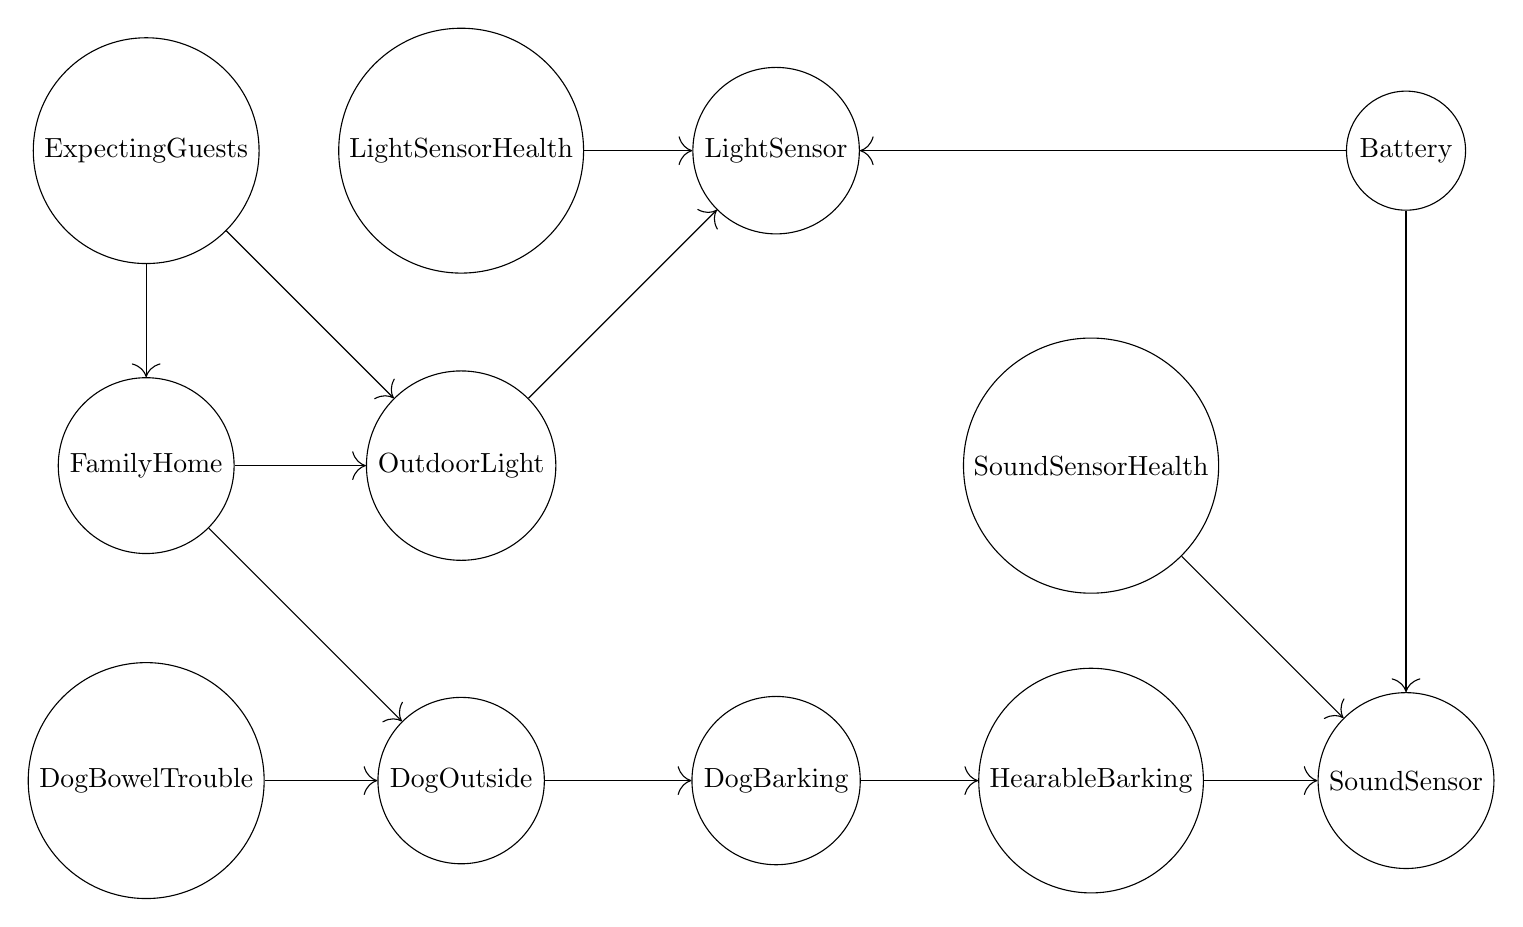
\begin{tikzpicture}
	\node[shape=circle,draw=black](EG) at (0,0) {ExpectingGuests};
	\node[shape=circle,draw=black](LSH) at (4,0) {LightSensorHealth};
	\node[shape=circle,draw=black](LS) at (8,0) {LightSensor};
	\node[shape=circle,draw=black](B) at (16,0) {Battery};
	\node[shape=circle,draw=black](FH) at (0,-4) {FamilyHome};
	\node[shape=circle,draw=black](OL) at (4,-4) {OutdoorLight};
	\node[shape=circle,draw=black](SSH) at (12,-4) {SoundSensorHealth};
	\node[shape=circle,draw=black](DBT) at (0,-8) {DogBowelTrouble};
	\node[shape=circle,draw=black](DO) at (4,-8) {DogOutside};
	\node[shape=circle,draw=black](DB) at (8,-8) {DogBarking};
	\node[shape=circle,draw=black](HB) at (12,-8) {HearableBarking};
	\node[shape=circle,draw=black](SS) at (16,-8) {SoundSensor};
	\path[-{>[scale=2]}](EG) edge node {} (FH)
		edge node {} (OL);
	\path[-{>[scale=2]}](LSH) edge node {} (LS);
	\path[-{>[scale=2]}](B) edge node {} (LS)
		edge node {} (SS);
	\path[-{>[scale=2]}](FH) edge node {} (OL)
		edge node {} (DO);
	\path[-{>[scale=2]}](OL) edge node {} (LS);
	\path[-{>[scale=2]}](SSH) edge node {} (SS);
	\path[-{>[scale=2]}](DBT) edge node {} (DO);
	\path[-{>[scale=2]}](DO) edge node {} (DB);
	\path[-{>[scale=2]}](DB) edge node {} (HB);
	\path[-{>[scale=2]}](HB) edge node {} (SS);
	\end{tikzpicture}
	\item Learn the network CPTs using the EM algorithm and the datafile (sambot.dat) available from the class homepage. Your intiial network should have uniform parameters.
	\end{enumerate}
You ned to turn in sambot.net and a report that contains the following information:
	\begin{itemize}
		\item The most likely instantiation of all variables given that Sambot has sensed the lights to be on, but has sensed no bark. Explain how you obtained this answer.
		\begin{enumerate}[label=\arabic*.]
			\item Construct causal structure.
			\item Run EM Learning with sambot.dat as the input data file.
			\item Set LightSensor to On and SoundSensor to Off.
			\item Run MPE.
		\end{enumerate}
		\[\begin{tabular} {|c|c|}
		\hline
		\textbf{Variable} & \textbf{Value} \\
		\hline
		Battery & OK \\
		\hline 
		DogBarking & No \\
		\hline
		DogBowelTrouble & Yes \\
		\hline
		DogOutside & Yes \\
		\hline
		ExpectingGuests & No \\
		\hline
		FamilyHome & No \\
		\hline
		HearableBarking & No \\
		\hline
		LightSensorHealth & OK \\
		\hline
		OutdoorLight & On \\
		\hline
		SoundSensorHealth & OK \\
		\hline
		\end{tabular}\]
		\item The most likely instantiation of the sensors given that the family is home and no guests are expected. Explain how you obtained this answer.
		\begin{enumerate}[label=\arabic*.]
			\item Construct causal structure.
			\item Run EM Learning with sambot.dat as the input data file.
			\item Set FamilyHome to Yes and ExpectingGuests to No.
			\item Run MPE.
		\end{enumerate}
		\[\begin{tabular} {|c|c|}
		\hline
		\textbf{Variable} & \textbf{Value} \\
		\hline
		LightSensor & Off \\
		\hline
		SoundSensor & Off \\
		\hline
		\end{tabular}\]
		\item The smallest set of variables \textbf{Z} in your network such that two sensors are independent given \textbf{Z}. Justify your answer based on d-separation.\\
		The set \{Battery, DogBowelTrouble\} is a set such that the two sensors are independent. Since the path\\DogBowelTrouble$\rightarrow$DogOutside$\rightarrow$DogBarking$\rightarrow$HearableBarking$\rightarrow$SoundSensor$\rightarrow$Battery$\rightarrow$LightSensor is blocked by Battery, this means that \{Battery, DogBowelTrouble\} d-separate the sensors, implying independence.
		\item The type of network you constructed: tree, polytree (singly-connected network), or multiply-connected network.\\
		\fbox{Multiply-connected network.}
	\end{itemize} 
\end{enumerate}
\end{document}